% =====================================================================
% Snippet: feedback-loop.tex
% =====================================================================
% USAGE: Feedback / autoregressive loop arrow that wraps around the
% right side of a block (e.g., Output Tokens → back to Start Token).
% Dashed purple, with rounded corners + label "prev. tokens".
%
% Used in: autoregressive decoders, RL training loops, GAN training.
%
% Copy %% COPY-START / END, replace:
%   - start_anchor: where the loop exits (e.g., output_box.east)
%   - end_anchor: where the loop returns (e.g., input_box.east)
%   - rail_x: x of the vertical rail (must be OUTSIDE other content)
%   - label: arrow label text
% =====================================================================

\documentclass[tikz,border=10pt]{standalone}
\usepackage{xcolor,tikz}
\usetikzlibrary{positioning,calc,arrows.meta,bending}

\definecolor{acaPurpleLine}{HTML}{6E3FA0}
\definecolor{acaPurpleFill}{HTML}{EDE3F6}
\definecolor{acaGreyLine}{HTML}{606060}
\definecolor{acaBlueLine}{HTML}{3060A8}
\definecolor{acaBlueFill}{HTML}{DCE6F4}

\tikzset{
  feedback arrow/.style={
    -{Stealth[length=5pt 1.2, width'=0pt 0.5]},
    line width=0.9pt, densely dashed,
    rounded corners=5pt,
    color=acaPurpleLine,
    shorten >=2pt, shorten <=2pt,
  },
}

\begin{document}
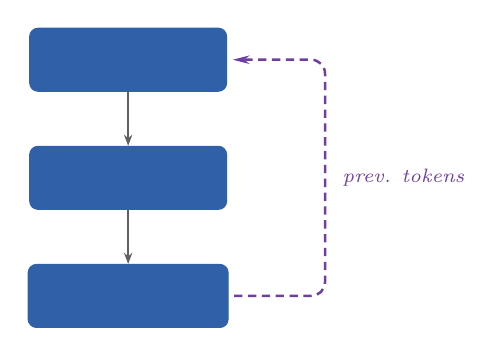
\begin{tikzpicture}

%% COPY-START =========================================================

% --- DEMO BOXES ---
\node[draw=acaBlueLine, fill=acaBlueFill, rounded corners=3pt,
      minimum width=2.5cm, minimum height=0.8cm,
      font=\small\bfseries, color=acaBlueLine]
  (input) at (0, 2.5) {Start Token};
\node[draw=acaBlueLine, fill=acaBlueFill, rounded corners=3pt,
      minimum width=2.5cm, minimum height=0.8cm,
      font=\small\bfseries, color=acaBlueLine]
  (decoder) at (0, 1.0) {Decoder};
\node[draw=acaBlueLine, fill=acaBlueFill, rounded corners=3pt,
      minimum width=2.5cm, minimum height=0.8cm,
      font=\small\bfseries, color=acaBlueLine]
  (output) at (0, -0.5) {Output Token};

% --- FORWARD ARROWS ---
\draw[-{Stealth[length=4pt]}, line width=0.8pt, color=acaGreyLine]
  (input.south) -- (decoder.north);
\draw[-{Stealth[length=4pt]}, line width=0.8pt, color=acaGreyLine]
  (decoder.south) -- (output.north);

% --- FEEDBACK LOOP: output → right rail → up → back to input ---
% Rail x is 1.0cm to the right of box right edge
\def\railX{2.5}            % x coordinate of vertical rail
\draw[feedback arrow]
  (output.east) -- (\railX, -0.5) -- (\railX, 2.5) -- (input.east);

% --- LABEL on the rail ---
\node[anchor=west, font=\scriptsize\itshape, color=acaPurpleLine]
  at (\railX + 0.1, 1.0) {prev. tokens};

%% COPY-END ===========================================================

\end{tikzpicture}
\end{document}
